\documentclass[a4paper,11pt,final]{article}
% Pour une impression recto verso, utilisez plutôt ce documentclass :
%\documentclass[a4paper,11pt,twoside,final]{article}

\usepackage[left=2cm,right=2cm,top=2cm,bottom=2cm]{geometry}
\usepackage[english,francais]{babel}
\usepackage[utf8]{inputenc}
\usepackage[T1]{fontenc}
\usepackage[pdftex]{graphicx}
\usepackage{setspace}
\usepackage{vmargin}
\usepackage{hyperref}
\usepackage[french]{varioref}

\usepackage{tocloft}
\addtocontents{toc}{\cftpagenumbersoff{section}}
\addtocontents{toc}{\cftpagenumbersoff{subsubsection}}

\newcommand{\reporttitle}{Algorithm Comparator}     % Titre
\newcommand{\reportauthor}{Nicolas \textsc{BÉDRINE}, Vincent \textsc{ALBERT}} % Auteur
\newcommand{\reportsubject}{Rapport de Projet de Découverte de la Recherche (PIDR)} % Sujet
\newcommand{\HRule}{\rule{\linewidth}{0.5mm}}
\setlength{\parskip}{1ex} % Espace entre les paragraphes

\hypersetup{
    pdftitle={\reporttitle},%
    pdfauthor={\reportauthor},%
    pdfsubject={\reportsubject},%
}

\begin{document}
  \newenvironment{changemargin}[2]{\begin{list}{}{%
\setlength{\topsep}{0pt}%
\setlength{\leftmargin}{0pt}%
\setlength{\rightmargin}{0pt}%
\setlength{\listparindent}{\parindent}%
\setlength{\itemindent}{\parindent}%
\setlength{\parsep}{0pt plus 1pt}%
\addtolength{\leftmargin}{#1}%
\addtolength{\rightmargin}{#2}%
}\item }{\end{list}}

\begin{titlepage}

\begin{flushleft}


\end{flushleft}

\begin{center}

\begin{minipage}[t]{0.48\textwidth}
  \begin{flushleft}
	
\includegraphics [width=50mm]{images/logo-telecom.png} \\[0.5cm]
      \textsc{\LARGE Telecom Nancy}
  \end{flushleft}
\end{minipage}
\begin{minipage}[t]{0.48\textwidth}
  \begin{flushright}
    
\includegraphics [width=50mm]{images/logo-ul.jpg} \\[0.5cm]
    \textsc{\LARGE Université de Lorraine}
  \end{flushright}
\end{minipage} \\[1.5cm]


	\textsc{\Large \reportsubject}\\[0.5cm]
	\HRule \\[0.4cm]
	{\huge \bfseries \reporttitle}\\[0.4cm]
	\HRule \\[1.5cm]
	
	\begin{minipage}[t]{0.3\textwidth}
 	 	\begin{flushleft} \large
  		\end{flushleft}
	\end{minipage}
	\begin{minipage}[t]{0.6\textwidth}
  		\begin{flushright} \large
    		\emph{Auteurs :} \\
    		Nicolas \textsc{Bédrine} \\
    		Vincent \textsc{Albert} \\
  		\end{flushright}
	\end{minipage}

\vfill

{\large \today{}}

\end{center}

\end{titlepage}

  \cleardoublepage % Dans le cas du recto verso, ajoute une page blanche si besoin
  \renewcommand\thepage{}
  \tableofcontents % Table des matières
  \sloppy          % Justification moins stricte : des mots ne dépasseront pas des paragraphes
  \cleardoublepage
  \renewcommand\thepage{\arabic{page}}
  \setcounter{page}{1}
  
  \section{Présentation du sujet} % Pas de numérotation
\addcontentsline{toc}{section}{Présentation du sujet} % Ajout dans la table des matières

\subsection{Un rapide résumé}

\begin{figure}[!ht]
    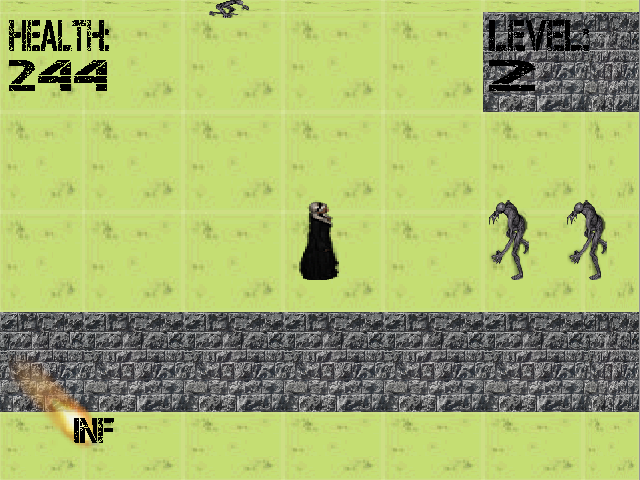
\includegraphics[width=0.5\textwidth]{./images/snapshot1.png}
    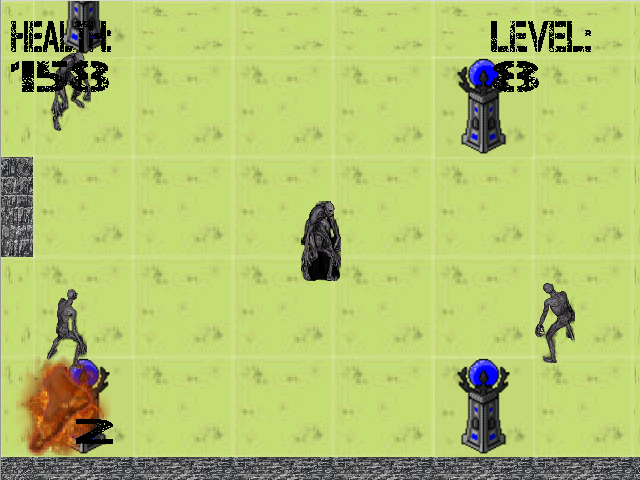
\includegraphics[width=0.5\textwidth]{./images/snapshot2.png}
    \caption{Snapshots}
\end{figure}

\subsection{Une licence pour les protéger tous}

Le logiciel et l'ensemble des sources sont sous licence CC BY-NC-SA 3.0 FR. Le partage et l'adaptation du logiciel sont permises à condition de ne pas l'utiliser
commercialement, d'indiquer les changements effectués, de référencer l’œuvre originale et 
de conserver la même licence.

\subsection{Le cahier des charges}
  \cleardoublepage
  \section{Organisation du projet}

\subsection{Les outils utilisés}


\subsection{Le planning initial}

Afin d'achever au mieux les objectifs que nous nous étions fixés, nous avons dressé un planning optimal des tâches à effectuer, en les répartissant par priorité. Voici le gantt des objectifs initiaux.

\begin{figure}[!ht]
    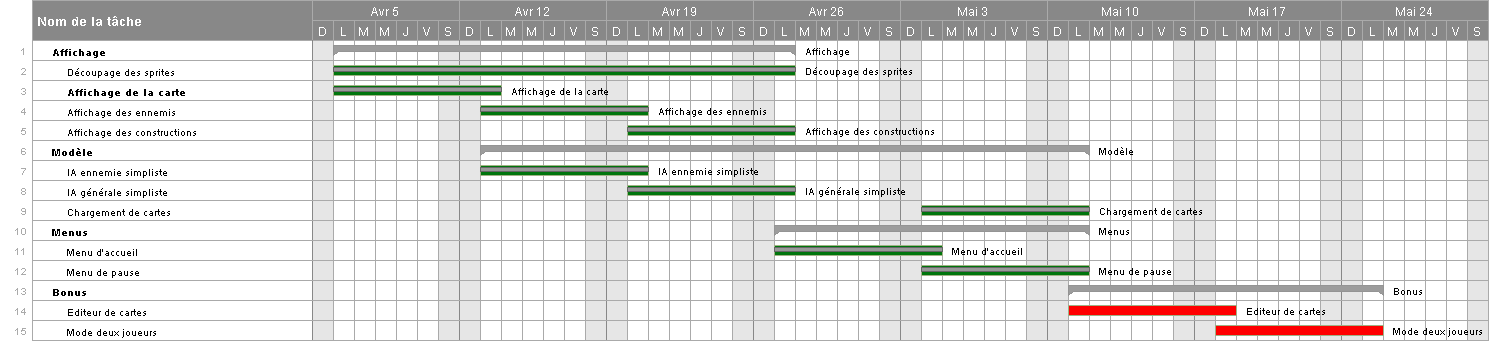
\includegraphics[width=1.1\textwidth]{./images/gantt.png}
    \caption{Gantt du projet}
\end{figure}

\subsection{UML des fichiers et fonctionnalités}

Voici le schéma simplifié de la structure des fichiers. Seuls les structures et fonctions les plus importantes ont été représentées afin de conserver la lisibilité du schéma. 

\begin{figure}[!ht]
    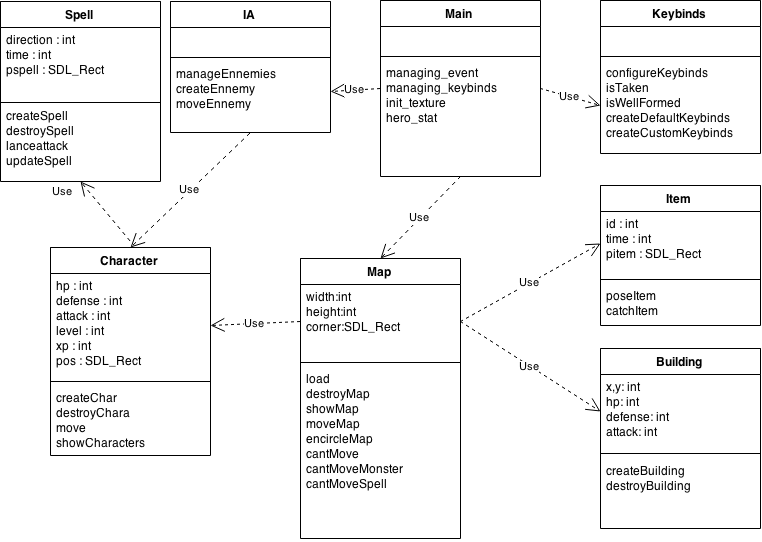
\includegraphics[width=1\textwidth]{./images/uml.png}
    \caption{UML}
\end{figure}

On peut remarquer l'organisation structurelle du code qui tend à se rapprocher d'un code objet. Les listes chaînées n'ont pas été représentées afin de ne pas encombrer l'UML.


  \cleardoublepage
  \section{La phase de développement}

\subsection{Les attentes atteintes}

\subsection{Ce qui pourrait être encore fait}

\subsection{Résultats d'expérience et interprétation}

\subsection{Les problèmes rencontrés}

	\subsubsection{De la refactorisation du modèle}
  \cleardoublepage
  
  \thispagestyle{empty}
  \section*{Références et autres sources d'inspiration}
\addcontentsline{toc}{section}{Références}

\url{http://blog.hikoweb.net/index.php?post/2011/11/06/Exemple-de-rapport-en-LaTeX} \\
\emph{Source pour le template \LaTeX ayant servi à la rédaction de ce rapport.} \\

\end{document}

